\pdfoutput=1
\documentclass[11pt]{amsart}
\usepackage{amsmath,amssymb,amsthm}
\usepackage[margin=1.2in]{geometry}
\usepackage{booktabs,adjustbox,graphicx,xcolor}
\usepackage[colorlinks=true,linkcolor=blue,citecolor=blue,urlcolor=blue]{hyperref}
\hypersetup{pdfauthor={Bernd Johannes Wuebben},
pdftitle={Metric wall crossing in rank-three K3 bundle moduli}}
\setlength{\emergencystretch}{2em}
\newtheorem{theorem}{Theorem}[section]
\newtheorem{proposition}[theorem]{Proposition}
\newtheorem{lemma}[theorem]{Lemma}
\newtheorem{corollary}[theorem]{Corollary}
\theoremstyle{definition}
\newtheorem{definition}[theorem]{Definition}
\newtheorem{example}[theorem]{Example}
\theoremstyle{remark}
\newtheorem{remark}[theorem]{Remark}
\newcommand{\CC}{\mathbb C}
\newcommand{\RR}{\mathbb R}
\newcommand{\PP}{\mathbb P}
\newcommand{\cO}{\mathcal O}
\newcommand{\cV}{\mathcal V}
\newcommand{\cQ}{\mathcal Q}
\newcommand{\cN}{\mathcal N}
\newcommand{\cM}{\mathcal M}
\newcommand{\cE}{\mathcal E}
\newcommand{\cD}{\mathcal D}
\newcommand{\ddbar}{\bar\partial}
\DeclareMathOperator{\tr}{tr}
\DeclareMathOperator{\Hom}{Hom}
\DeclareMathOperator{\End}{End}
\DeclareMathOperator{\Ext}{Ext}
\DeclareMathOperator{\Gr}{Gr}
\DeclareMathOperator{\rank}{rank}
\DeclareMathOperator{\im}{im}
\DeclareMathOperator{\arsinh}{arsinh}
\DeclareMathOperator{\diag}{diag}
\DeclareMathOperator{\Vol}{Vol}
\title[Metric wall crossing in K3 bundle moduli]{Metric wall crossing in rank-three K3 bundle moduli}
\author{Bernd Johannes Wuebben}
\subjclass[2020]{14J60, 53C07 (primary); 14J28, 14D20, 53C26 (secondary)}
\keywords{K3 surface, bundle moduli, Hermitian--Einstein metric, stability wall,
hyperk\"ahler quotient, stratified Mukai flop}
\date{November 6, 2026}
\begin{document}
\begin{abstract}
We determine the local harmonic $L^2$ metric near a stability wall in a
complex twelve-dimensional moduli space of rank-three bundles on a
projective K3 surface. The central bundle is the sum of two copies of one
spherical line bundle and a second spherical line bundle, with
five-dimensional cross-extension spaces; the central K\"ahler metric is
Ricci-flat. We compare the actual chamber metrics with the standard
hyperk\"ahler quotient metrics on $T^*\Gr(2,5)$ and $T^*\Gr(3,5)$, with
relative error quadratic in the deformation size. The comparison is
uniform through changes of stabilizer and permits unrelated rates of
approach to the wall and its singular strata. It gives the exceptional-fibre
collapse scale, complete pointed Gromov--Hausdorff limits after rescaling,
quantitative matching to the wall metric, and intrinsic distance
asymptotics to the contracted loci. The proof corrects the real moment
equation within complex orbits with a bound that remains uniform at the
reducible strata.
\end{abstract}
\maketitle
\section{Introduction}\label{sec:introduction}

Variation of stability changes the birational geometry of moduli spaces
of sheaves on a K3 surface. Near a polystable sheaf, an Ext-quiver can
describe the analytic contraction and its exceptional strata. On the
locally free locus, the Hermitian--Einstein correspondence gives another
geometric structure: a tangent vector has the $L^2$ norm of its harmonic
Kodaira--Spencer representative. An analytic quiver description does not
identify this metric. In particular, it does not determine its behavior
when several exceptional strata approach one another at different rates.

We establish such a metric comparison for a rank-three wall crossing whose
local complex geometry is the stratified Grassmannian Mukai flop. The wall
contains an eight-dimensional stratum with projective-plane fibres and a
more reducible point with a Grassmannian fibre. The comparison holds on a
full neighborhood containing both strata. It gives relative asymptotics
for intrinsic distances, the complete metric obtained by rescaling the
contracting region, and a quantitative comparison with the surrounding
wall metric.

\subsection{The moduli problem and metric convention}

Section~\ref{sec:k3} constructs a smooth genus-four K3 surface $X$ containing
smooth rational curves $D_1,D_2$ such that
\begin{equation}\label{eq:intersection-intro}
D_1^2=D_2^2=-2,\qquad D_1D_2=5,\qquad H=D_1+D_2\ \text{is ample}.
\end{equation}
Put $L_i=\cO_X(D_i)$ and
\[
E_0=(L_1\otimes\CC^2)\oplus L_2,\qquad
v=(3,2D_1+D_2,0),\qquad D=D_1-D_2.
\]
We fix the holomorphic determinant $L_1^2L_2$. The Mukai vector $v$ is
primitive, $v^2=10$, and $c_2(E_0)=8$. At the polarization $H$, the
bundle $E_0$ is both slope-polystable and Gieseker-polystable.

Choose a smooth path of K\"ahler forms $\omega_t$ in $H+tD$, for $|t|$
small, with $\omega_0$ Ricci-flat, whose existence in $H$ follows from
Yau's theorem \cite{Yau78}. Let
$\cM_t^{\rm bun}$ be the moduli space of slope-polystable locally free
bundles of vector $v$ and the specified determinant. We use its
Hermitian--Yang--Mills connection topology. On each smooth orbit-type
stratum, where the conjugacy class of the effective compact stabilizer
is fixed, its metric $g_t$ is the harmonic Dolbeault metric, with
\begin{equation}\label{eq:dolbeault-norm}
\|a\|_{\omega_t,h}^2
=\int_X\tr(i a^\dagger\wedge a)\wedge\omega_t .
\end{equation}
There is no division by volume. The real connection variation $a-a^\dagger$
has squared norm twice~\eqref{eq:dolbeault-norm}. The determinant line has
its $\omega_t$-Hermitian--Einstein metric; changing a scalar bundle metric
does not affect the endomorphism norms in~\eqref{eq:dolbeault-norm}.

The length distance $d_t$ is defined using continuous paths that are
piecewise smooth on the smooth orbit-type strata, with local gauge
lifts. Finite-length limiting endpoints at lower strata are allowed.
Paths used to define $d_t$ may leave any prescribed coordinate
neighborhood; they remain in the locally free moduli component. We do
not impose this metric on non-locally-free sheaves.

\subsection{The comparison theorem}

We first specify the finite-dimensional quotient metric appearing in the result. Let
\[
\cV=\Hom(\CC^2,\CC^5)\oplus\Hom(\CC^5,\CC^2),\qquad x=(A,B),
\]
with Euclidean Hermitian norm $\|x\|^2=\tr A^*A+\tr BB^*$.
The group $G=GL_2(\CC)$ acts by
$(A,B)\mapsto(Ag^{-1},gB)$, with compact form $K=U(2)$. Define
\begin{equation}\label{eq:model-intro}
M_\tau=\{BA=0,\ A^*A-BB^*=\tau I_2\}/K,\qquad
\tau=\tau(t)=-\frac{28\pi}{3}t .
\end{equation}
Write $g_\tau^{\rm q}$ and $d_\tau^{\rm q}$ for its flat quotient metric
and length distance, and $r_\tau([A,B])=(\|A\|^2+\|B\|^2)^{1/2}$.
At $\tau=0$ these are understood on the stratified quotient.

The invariant $N=AB$ takes values in
\begin{equation}\label{eq:nilpotent-cone}
\cN=\{N\in\End(\CC^5):N^2=0,\ \rank N\le2\}.
\end{equation}
For $\tau>0$, $M_\tau=T^*\Gr(2,5)$; for $\tau<0$,
$M_\tau=T^*\Gr(3,5)$; and $M_0=\cN$. The quotient maps
$\pi_\tau:M_\tau\to\cN$ are the two incidence resolutions. Their fibres
are points over rank two, $\PP^2$ over rank one, and the full
Grassmannians over zero. Section~\ref{sec:model} recalls these
identifications with their metric normalizations.

\begin{theorem}\label{thm:main}
There are $R,t_0,C>0$ such that, for $|t|<t_0$, there are
homeomorphisms
\[
f_t:\{r_{\tau(t)}<R\}\subset M_{\tau(t)}
\longrightarrow U_t\subset\cM_t^{\rm bun}
\]
onto open subsets. They are smooth and biholomorphic on the corresponding
smooth complex orbit-type strata. The vertex maps to $[E_0]$ at
$t=0$, and the whole zero section is included for all sufficiently small
nonzero $t$. Every point of $U_t$ is slope-stable when $t\ne0$.

On every smooth piece and for every tangent vector,
\begin{equation}\label{eq:main-tensor}
(1-C(|t|+r_\tau^2))g_\tau^{\rm q}
\ \le\ f_t^*g_t\ \le\
(1+C(|t|+r_\tau^2))g_\tau^{\rm q}.
\end{equation}
The constants are independent of the positive singular values of $AB$
and of their ratios to each other and to $|t|$.

For some $c,C'>0$, if $r_\tau(p),r_\tau(q)\le\rho\le cR$, then
\begin{equation}\label{eq:main-distance}
(1-C'(|t|+\rho^2))d_\tau^{\rm q}(p,q)
\le d_t(f_t(p),f_t(q))
\le(1+C'(|t|+\rho^2))d_\tau^{\rm q}(p,q).
\end{equation}
The middle distance allows paths throughout the locally free moduli
component.
\end{theorem}

The parameter in~\eqref{eq:model-intro} follows from the Chern degrees and
the harmonic pairing; it is not a choice of scaling exponent. Since
$r_\tau^2\ge2|\tau|$, the error in~\eqref{eq:main-tensor} is also $O(r_\tau^2)$.
At the wall, the rank-one piece parametrizes bundles $L_1\oplus F$, where
$F$ is stable of Mukai vector $(2,H,0)$. It meets the more reducible
bundle $E_0$. Thus the uniformity includes a genuine change from effective
circle symmetry to effective $U(2)$ symmetry.

For the integral ample classes $mH\pm D$, with $m$ sufficiently large,
$c_1(E_0)(mH\pm D)=9m\mp7$ is coprime to three. Slope and Gieseker
stability therefore coincide for these invariants. The two chamber
neighborhoods occur in the locally free loci of the ordinary projective
sheaf moduli spaces. The contraction diagram asserted here is local
and analytic. It does not require a global morphism to the ordinary
$H$-Gieseker wall moduli space.

\subsection{Distances and rescaled geometry}

Let $s_1\ge s_2\ge0$ be the singular values of $N=AB$. For $\kappa>0$ set
\begin{equation}\label{eq:profile-intro}
b_i^2=\frac{\sqrt{\kappa^2+4s_i^2}-\kappa}{2},\qquad
F_\kappa(b)=\int_0^b
\sqrt{\frac{\kappa+2u^2}{\kappa+u^2}}\,du.
\end{equation}
For $\kappa=0$ put $b_i=\sqrt{s_i}$ and $F_0(b)=\sqrt2\,b$.
Take a slightly larger chart than the one in Theorem~\ref{thm:main},
so that closed radius subsets are defined. Let
\[
\cE_t=f_t(\pi_\tau^{-1}(0)),\qquad
\cD_t=f_t(\pi_\tau^{-1}\{\rank N\le1\}\cap\{r_\tau\le R\}).
\]
These are the deepest fibre and the local contracted locus; at $t=0$
they become the vertex and the closure of the reducible stratum.

\begin{theorem}\label{thm:distances}
For $x$ of radius $r=r_\tau(x)\le cR$, with $\kappa=|\tau|$,
\begin{align}
d_t(f_t(x),\cE_t)
&=(1+O(|t|+r^2))
\sqrt{F_\kappa(b_1)^2+F_\kappa(b_2)^2},\label{eq:distance-zero}\\
d_t(f_t(x),\cD_t)
&=(1+O(|t|+r^2))F_\kappa(b_2).\label{eq:distance-rank}
\end{align}
The errors are multiplicative and uniform in all the indicated scales.
At zero distance the formulas mean equality to zero.

The metric induced on $\cE_t$ is $|\tau|$ times the standard
Grassmannian quotient metric, with relative error $O(|t|)$.
On the $\PP^2$ fibre over a rank-one matrix of singular value $s>0$,
the induced metric is $|\tau|$ times the Hopf-quotient Fubini--Study
metric, with relative error $O(|t|+s)$.
\end{theorem}

In particular,
\[
d_0(f_0(N),\cD_0)=(1+O(r_0^2))\sqrt{2s_2}.
\]
For nonzero $\tau$, the exact model profile crosses from
$s_2/\sqrt{|\tau|}$ when $s_2\ll|\tau|$ to $\sqrt{2s_2}$ when
$|\tau|\ll s_2$. Formula~\eqref{eq:distance-rank} controls the
intermediate ratios and remains relative even if this distance is
arbitrarily small compared with $r$. Fibre metrics in the theorem are
induced metrics; their intrinsic distances are not identified with
unrestricted ambient distances between fibre points.

\begin{corollary}\label{cor:limits}
Fix a zero-section point in $M_{+1}$ or $M_{-1}$. On the corresponding
side of the wall, dividing $g_t$ by $\kappa=|\tau(t)|$ gives the complete
pointed length-space limit
$(M_{+1},g_{+1}^{\rm q})$ or $(M_{-1},g_{-1}^{\rm q})$.
More precisely, the maps
$\iota_t(\widehat x)=f_t(\sqrt\kappa\,\widehat x)$ satisfy
\begin{equation}\label{eq:inner-intro}
(1-C\kappa(1+\widehat r^2))g_{\pm1}^{\rm q}
\le\kappa^{-1}\iota_t^*g_t
\le(1+C\kappa(1+\widehat r^2))g_{\pm1}^{\rm q}.
\end{equation}
This holds on expanding domains $\widehat r\le R_t$ whenever
$R_t\to\infty$ and $\kappa R_t^2\to0$, and implies pointed
Gromov--Hausdorff convergence on every bounded pointed ball.

On the common rank-two locus, using $N$ to identify the chamber with
the wall, the actual chamber and wall metrics have relative difference
\begin{equation}\label{eq:outer-intro}
O\left(|t|+r_0^2+\frac{|\tau|}{s_2}\right)
\end{equation}
when $|\tau|/s_2$ is sufficiently small.
\end{corollary}

The abstract Riemannian spaces $M_{+1}$ and $M_{-1}$ are isometric
by adjoint interchange. Their contractions over the fixed matrix $N$
are different. The complete metrics in the corollary are classical;
the assertion identifies them as limits of the actual harmonic metric.
Neither the corollary nor the tensor estimate asserts smooth convergence
or curvature bounds.

\subsection{Relation to previous work and the analytic argument}

The complex geometry uses established K3 deformation theory. Budur--Zhang
\cite[Theorem~1.2]{BZ19} prove formality for a sheaf polystable with
respect to any ample polarization. Arbarello--Sacc\`a
\cite[Propositions~4.4 and~6.1]{AS18} give the equivariant analytic
quadratic germ and its quiver interpretation. Their adjacent-polarization
wall-crossing theorem concerns pure one-dimensional sheaves; it is not
used for the rank-three bundles here. Buchdahl--Schumacher
\cite{BS21,BS22} construct harmonic analytic deformation quotients.
Delloque's simultaneous deformation theory
\cite[Propositions~4.3--4.6 and Theorem~7.4]{Del25}
supplies corrected HYM equations and an open actual moduli neighborhood
on the integrable locus, without an abelian-stabilizer assumption.

Local metric comparison in reduction is also not new. Sjamaar
\cite[arXiv version, Lemma~2.13 and its proof]{Sja95} compares the reduced
K\"ahler metric with its flat holomorphic slice metric on the top stratum
near a chosen quotient point. Sjamaar--Lerman's singular-reduction theory
\cite{SL91}, using the classical symplectic normal form, and Mayrand's
complex Hamiltonian normal form \cite[Theorems~1.3 and~1.4]{May22}
preserve structures different from the full Riemannian metric. A real symplectic
coordinate change need not preserve an independently imposed complex
integrability equation. Namikawa--Odaka \cite[Remark~6.14]{NO26}
discuss the stronger metric comparison problem in the setting of
symplectic singularities; their isolated-singularity and finite
hyperk\"ahler quotient results do not directly give the simultaneous
estimate in Theorem~\ref{thm:main}.

The complete cotangent-Grassmannian metric and its quotient description
are classical \cite{BG96}. Qualitative Gromov--Hausdorff continuity
through suitable projective Calabi--Yau flops is proved by Rong--Zhang
\cite[Theorem~1.2]{RZ11}. Actual Weil--Petersson forms on bundle moduli
and their extensions are studied in \cite{BS21,BS23}; explicit metrics
and degenerations for framed bundles on the blown-up plane appear in
\cite{BS26}. Gauge slices and reduction by the residual finite-dimensional
group are part of the earlier Yang--Mills moduli theory
\cite{GP89}. We do not claim these constructions or the finite
Grassmannian scaling as new.

The additional issue is to compare the \emph{actual} real moment levels
on the exact obstructed complex locus, with an error independent of the
smallest positive infinitesimal gauge direction. A usual implicit-function
bound can lose that direction. We replace it by a projection estimate.
If $\mu=A^*A-BB^*$ and $\rho$ is the centered corrected moment map,
then for every orthogonal projection $P$ on $\CC^2$,
\[
|\tr(P(\rho-\mu))|
\le\epsilon\bigl(\|AP\|^2+\|PB\|^2\bigr).
\]
The right side is the squared norm of the circle action generated by
$P$. Testing this estimate on spectral projections of the positive
Hermitian factor of a complex gauge transformation bounds that factor
uniformly through rank loss. Projection-relative curvature estimates and
finite-dimensional balancing by spectral projections were developed for
repeated stable factors in \cite{Wue26a,Wue26c}. Here we adapt this method
to the exact obstructed K3 deformation locus and compare different real
moment levels. Section~\ref{sec:balancing} gives the required argument
in full.

The harmonic norm requires a separate identification. We first minimize
over the uniformly coercive complement of the parallel gauge algebra,
as in the complementary-gauge method of \cite{Wue26b}. The result is a
smooth positive Hermitian form on the full deformation space. A central
automorphism acting by minus the identity removes its linear term.
Only then do we minimize over the remaining complex orbit directions.
Derivatives of the real balancing transformation are exact gauge terms
and disappear from that infimum. Finally, a radius estimate excludes
shorter paths leaving the chart. These steps give the actual intrinsic
conclusions, rather than merely a comparison of norms on an assumed
common locus.

The result is local and concerns locally free bundles. It gives no
global completion theorem, no bubbling description, and no general
metric normal-form theorem for hyperk\"ahler singularities.

The polynomial calculations of Section~\ref{sec:k3} and the distance
profile in Figure~\ref{fig:distance} can be reproduced from the
source accompanying this paper at
\url{https://github.com/bwuebben/stability-degeneration}.

\section{A K3 surface and its stability wall}\label{sec:k3}

\subsection{An explicit surface}

In $\PP^4$ with coordinates $[x_0:\cdots:x_4]$, put
\begin{align}
q&=x_0x_3-x_1x_2+x_4^2,\nonumber\\
c_0&=x_0^3+x_0x_1^2+2x_0x_2^2+5x_1x_2x_3
       +4x_0x_1x_2+3x_1^2x_3+2x_2^2x_3,\label{eq:k3-polynomials}\\
c&=c_0+x_4(x_0^2+x_3^2+x_4^2),\qquad X=V(q,c).\nonumber
\end{align}

\begin{proposition}\label{prop:k3}
The surface $X$ is a smooth K3 surface. Its hyperplane section $x_4=0$
is the union of two smooth rational curves satisfying
\eqref{eq:intersection-intro}.
\end{proposition}

\begin{proof}
The quadratic form is nondegenerate, and $c$ is not divisible by $q$.
Smoothness can be checked by the following exact finite computation.
Over $\mathbb F_{101}$, take the ideal generated by $q,c$ and the ten
$2\times2$ minors of their Jacobian. On each affine chart $x_i=1$,
its reduced Gr\"obner basis is
\[
\begin{array}{c|ccccc}
i&0&1&2&3&4\\ \hline
\text{basis}&[1]&[1]&[1]&[1]&[1].
\end{array}
\]
All the polynomial inputs are printed in~\eqref{eq:k3-polynomials};
the accompanying calculation constructs the minors and uses exact
arithmetic in $\mathbb F_{101}$. Thus the geometric singular subscheme
in that fibre is empty, not merely its set of rational points.
The projective Jacobian subscheme over $\operatorname{Spec}\mathbb Z$
is proper. If its generic fibre were nonempty, its closed image would
contain the generic point and hence every prime, a contradiction at
101. The characteristic-zero Jacobian criterion proves smoothness.
Adjunction gives $K_X=\cO_X$, and the complete-intersection cohomology
sequence gives $H^1(X,\cO_X)=0$. Hence $X$ is K3.

On $q=x_4=0$ use Segre coordinates
$[x_0:x_1:x_2:x_3]=[au:av:bu:bv]$. The cubic restricts to $fg$, where
\begin{equation}\label{eq:two-curves}
f=a(u^2+v^2)+buv,\qquad
g=(a^2+2b^2)u+3abv.
\end{equation}
The two coefficients in each linear expression have no common zero.
Thus $D_1=V(f)$ and $D_2=V(g)$ are smooth rational graphs of bidegrees
$(1,2)$ and $(2,1)$ on $\PP^1\times\PP^1$.
On $a=u=1$, their intersection has
\[
-z^4+2z^2+2=0,\qquad b=-\frac{1+z^2}{z},\qquad z=v.
\]
There are four distinct nonzero roots. The fifth intersection has
$[a:b]=[u:v]=[0:1]$. In the chart $b=v=1$, substitution
$a=-u/(1+u^2)$ into $g$ has leading term $-u$, proving transversality
there. These exhaust the intersection number.

At a finite intersection, the normal derivative of $c$ is
$x_0^2+x_3^2=1+(1+z^2)^2=4(1+z^2)$ modulo the quartic, hence is
nonzero. At the fifth point it is one. The intersections are therefore
transverse also as curves on $X$. Their sum is the hyperplane section,
which is ample. Adjunction gives $D_i^2=-2$, and the five crossings give
$D_1D_2=5$. In particular $H^2=6$ and $HD_i=3$.
\end{proof}

There is also a noncomputational existence argument for the same
configuration. On the smooth quadric threefold $V(q)$, lift a product
section of bidegree $(3,3)$ from the hyperplane quadric. Vary its lift by
$x_4G$, where $G$ is quadratic. This linear variation is base-point-free
off the hyperplane, so a general member is smooth there by Bertini.
Along either component away from its transverse crossings, the
tangential derivative is nonzero. At the finitely many crossings, avoid
the finitely many affine hyperplanes on which the normal derivative
vanishes. The explicit equations above select one smooth member; no
assumption on the full Picard group of that member is needed.

\subsection{Bundles, obstruction and polarization}

For the Mukai convention $v(F)=(r,c_1,r+c_1^2/2-c_2)$,
\begin{equation}\label{eq:mukai-data}
v(L_i)=(1,D_i,0),\quad
v(E_0)=(3,2D_1+D_2,0),\quad c_2(E_0)=8,\quad v(E_0)^2=10.
\end{equation}
The class $2D_1+D_2$ pairs to one with $D_1$, so it is primitive.
The stable K3 moduli dimension is $v^2+2=12$
\cite{Muk84}. Nonemptiness in the chambers will follow from the
actual local construction, rather than from the dimension formula.

The line bundles have $H$-degree three and Euler characteristic one.
They are stable for every polarization, and their reduced $H$-Hilbert
polynomials agree. The differences $\pm(D_1-D_2)$ are nonzero classes
of $H$-degree zero and cannot be effective. Therefore
\[
\Hom(L_1,L_2)=\Hom(L_2,L_1)=0.
\]
Serre duality gives vanishing of both cross $\Ext^2$ groups.
Since $(D_1-D_2)^2=-14$, Riemann--Roch gives
\begin{equation}\label{eq:ext-dimensions}
\dim\Ext^1(L_1,L_2)=\dim\Ext^1(L_2,L_1)=5,\qquad
\Ext^1(L_i,L_i)=0.
\end{equation}
Serre-dual bases identify $\Ext^1(E_0,E_0)$ with $\cV$.
The quadratic Yoneda obstruction has blocks $-BA$ and $\tr(BA)$,
up to a common nonzero scalar; its zero locus is $BA=0$.
Section~\ref{sec:coordinates} establishes both harmonic normalization
of these bases and the convergent comparison with the full reduced
integrability germ.

The effective automorphism group is
$(GL_2\times GL_1)/\CC^*\simeq GL_2$.
The determinant-one group is a finite cover with an ineffective
$\mu_3$ center. A trivial effective stabilizer will mean simplicity of
the bundle, not literal absence of determinant-one scalar automorphisms.

For the ample real class $H_t=H+tD$, one has
\begin{align}
H_t^2&=6-14t^2,\nonumber\\
\mu_t(L_1)&=3-7t,\qquad \mu_t(L_2)=3+7t,\qquad
\mu_t(E_0)=3-\tfrac73t,\label{eq:slopes}\\
\mu_t(L_1)-\mu_t(E_0)&=-\tfrac{14}{3}t,\qquad
\mu_t(L_2)-\mu_t(E_0)=\tfrac{28}{3}t.\nonumber
\end{align}
Thus the slope ordering changes transversely. If $m$ is sufficiently
large, $mH\pm D$ is integral ample and
$c_1(E_0)(mH\pm D)=9m\mp7$ is coprime to three.
Equality of slopes with a subsheaf of rank one or two would force that
rank to be divisible by three. The standard implications between
slope and Gieseker stability then identify all the stable and
semistable loci for these rank-three invariants.
This arithmetic does not itself give a wall contraction; the local
HYM construction below supplies that identification.

\section{The Grassmannian quotient and its distances}\label{sec:model}

The complete hyperk\"ahler metric on a cotangent Grassmannian is
classical. The conventions below agree with the quotient construction
in \cite[\S2.2]{BG96}, where the real parameter is written $2k$.
We give the calculations needed for the metric comparison and distance
statements, including their behavior at smaller rank.

\subsection{Quotients, radii and strata}

Use $\cV,G,K$ from Section~\ref{sec:introduction}, and write
$g^{\rm amb}$ for its Euclidean real metric. For $h\in\operatorname{Herm}_2$,
the compact fundamental vector and its complex rotation are
\begin{equation}\label{eq:fundamental}
\xi_h=(-Aih,ihB),\qquad I\xi_h=(Ah,-hB).
\end{equation}
With $\omega^{\rm amb}(v,w)=g^{\rm amb}(Iv,w)$,
\[
d\tr(\mu h)(v)=2\omega^{\rm amb}(\xi_h,v),\qquad
\mu=A^*A-BB^*.
\]
The complex moment equation is $BA=0$.

\begin{proposition}\label{prop:finite-geometry}
The spaces $M_\tau$ have the incidence presentations stated in the
introduction. For $\tau\ne0$ they are smooth complete hyperk\"ahler
manifolds. The rank-$k$ stratum of $M_0=\cN$ has complex dimension
$2k(5-k)$ for $k=0,1,2$. If $s_1\ge s_2\ge0$ are the singular values
of $N$, then
\begin{equation}\label{eq:radius}
r_\tau^2=\sum_{i=1}^2\sqrt{\tau^2+4s_i^2}.
\end{equation}
The dilation $x\mapsto ax$ sends $\tau$ to $a^2\tau$, $N$ to $a^2N$,
and the quotient metric to $a^2g_\tau^{\rm q}$.
\end{proposition}

\begin{proof}
For $\tau>0$, $A$ is injective. Its image $U$ is a two-plane, and
$BA=0$ gives
$\im N\subset U\subset\ker N$. Conversely, fix such $(U,N)$ and choose
an isometric frame $U_0:\CC^2\to U$. Write $N=U_0C$, so $CU_0=0$.
Set
\begin{equation}\label{eq:positive-representative}
P=\frac{\tau I+\sqrt{\tau^2I+4CC^*}}2,\qquad
A=U_0P^{1/2},\qquad B=P^{-1/2}C.
\end{equation}
Then $BA=0$, $AB=N$, and $A^*A-BB^*=\tau I$.
Conversely, the polar decomposition of any balanced $A$ yields this
formula, since $P(P-\tau I)=CC^*$ has the displayed unique positive
solution. Changing the frame changes the representative by $K$.
The incidence variety is $T^*\Gr(2,5)$.
The adjoint interchange $(A,B)\mapsto(B^*,A^*)$ exchanges $\tau$ with
$-\tau$ and gives the analogous presentation with a three-plane
between $\im N$ and $\ker N$.

At zero level, $A^*A=BB^*=P$. On its support, polar decomposition gives
$A=U_0P^{1/2}$ and $B=P^{1/2}V_0^*$, with $V_0^*U_0=0$.
Thus $N=U_0PV_0^*$ determines its balanced compact orbit. Conversely,
a singular-value decomposition of any square-zero matrix of rank at
most two has this form and supplies a zero-level representative.
The invariant ring is generated by the entries of $AB$, by the first
fundamental theorem for $GL_2$ \cite[\S2.1--2.2]{KP96}.
Restriction to the reduced invariant subvariety $BA=0$ preserves these
generators, by the Reynolds projection. Its image is exactly
\eqref{eq:nilpotent-cone}, so the reduced affine quotient is $\cN$.
This argument does not require an unproved normality assertion.

At rank two the incidence planes are $\im N$ and $\ker N$.
At rank one they are respectively a line and a two-plane in
$\ker N/\im N\simeq\CC^3$, giving two dual projective planes.
At zero they are the whole Grassmannians. Counting a flag
$\im N\subset\ker N$ and the induced isomorphism
$\CC^5/\ker N\to\im N$ gives dimension $2k(5-k)$.

For nonzero $\tau$ the effective compact action is free. The complex
equation has surjective differential when $A$ is injective or $B$
surjective, and the real moment has full transverse rank. Thus the
quotient is smooth. The level is closed in Euclidean space, and its
compact quotient with the induced length metric is complete: a
finite-length escaping path would have bounded Euclidean radius and
hence an endpoint in a compact part of the level quotient.

The eigenvalues of $P+BB^*$ are
$\sqrt{\tau^2+4s_i^2}$, proving~\eqref{eq:radius}. The dilation
assertions follow directly from the quadratic equations and Euclidean
metric.
\end{proof}

The two incidence maps over the same $N$ are distinct, although adjoint
interchange is an isometry between the abstract Riemannian spaces at
opposite parameters. Their complex dimensions are twelve. At zero
the radius is $r_0^2=2(s_1+s_2)$.

\subsection{Exact model distances}

Let $E_\tau=\pi_\tau^{-1}(0)$ and
$D_\tau=\pi_\tau^{-1}\{\rank N\le1\}$, including the zero-level meanings.
Use $b_i,F_\kappa$ from~\eqref{eq:profile-intro}.

\begin{proposition}\label{prop:model-distances}
For the full quotient length spaces,
\begin{equation}\label{eq:model-distances}
d_\tau^{\rm q}(x,E_\tau)
=\sqrt{F_\kappa(b_1)^2+F_\kappa(b_2)^2},\qquad
d_\tau^{\rm q}(x,D_\tau)=F_\kappa(b_2),\quad \kappa=|\tau|.
\end{equation}
Both distances have minimizing paths along which $r_\tau$ decreases.
\end{proposition}

\begin{proof}
First take $\tau>0$. Diagonalize $BB^*$ in the polar frame of $A$.
There are orthogonal isometric two-frames $U,V$ with
\[
A=U\diag(a_1,a_2),\quad
B=\diag(b_1,b_2)V^*,\quad
a_i=\sqrt{\tau+b_i^2}.
\]
If a $b_i$ vanishes, fill out the corresponding frame in $U^\perp$,
which has dimension three. Then $s_i=a_ib_i$, giving the expression
for $b_i$ in~\eqref{eq:profile-intro}.

The Frobenius singular-value inequality \cite{Mir60}
$\sum_i|\sigma_i(X)-\sigma_i(Y)|^2\le\|X-Y\|^2$
implies that ordered singular values along an absolutely continuous
matrix path are absolutely continuous, with their squared speeds
bounded by the squared matrix speed. Applying it to $A$ and $B$ yields
\begin{equation}\label{eq:singular-speed}
\|\dot A\|^2+\|\dot B\|^2
\ge\sum_i(\dot a_i^2+\dot b_i^2)
=\sum_i\left|\frac{d}{du}F_\tau(b_i)\right|^2
\end{equation}
almost everywhere. Difference quotients prove this also at collisions;
no smooth choice of singular vectors is assumed. Compact gauge changes
preserve all the singular values, so horizontal minimization proves that
$x\mapsto(F_\tau(b_1),F_\tau(b_2))$ is 1-Lipschitz for quotient
length. Its value on $E_\tau$ is zero, and its second component
vanishes on $D_\tau$. This proves both lower bounds.

For the first upper bound, keep $U,V$ fixed and set
$F_\tau(b_i(u))=uF_\tau(b_i(1))$ for $0\le u\le1$.
Choose $a_i(u)=\sqrt{\tau+b_i(u)^2}$. The path stays on both moment
equations and has constant ambient speed equal to the first expression
in~\eqref{eq:model-distances}. It ends on $E_\tau$. For the second
upper bound, keep $b_1$ fixed and vary only $b_2$ in this way.
The radii decrease. Their real diagonal velocities are also
compact-horizontal, although the ambient length upper bound already
suffices.

For $\tau<0$ use adjoint interchange. For $\tau=0$, $a_i=b_i=\sqrt{s_i}$
and $F_0(b_i)=\sqrt2\,b_i$; the same paths reach lower strata in
finite length. Inequality~\eqref{eq:singular-speed} holds on the
pieces and passes to the limiting endpoints. Hence no path through a
lower stratum shortens the displayed lower bounds.
\end{proof}

The scaling identity is $F_\kappa(\sqrt\kappa\,b)=\sqrt\kappa\,F_1(b)$.
Consequently $F_\kappa(b_2)\sim s_2/\sqrt\kappa$ if $s_2/\kappa\to0$,
and $F_\kappa(b_2)\sim\sqrt{2s_2}$ if $s_2/\kappa\to\infty$.
The full profile, rather than either asymptotic alone, is used below.

\begin{figure}[tb]
\centering
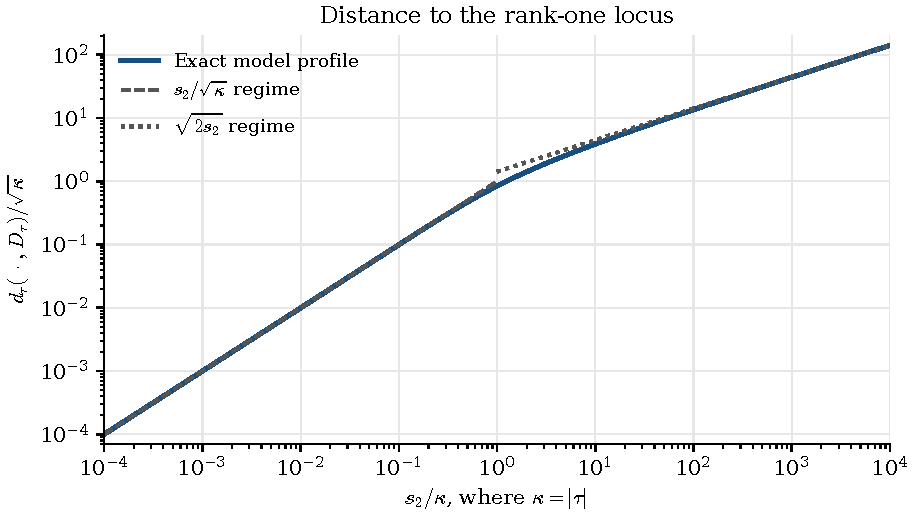
\includegraphics[width=.94\textwidth]{figures/distance-profile.pdf}
\caption{The exact model distance to $D_\tau$, divided by
$\sqrt{\kappa}$, as a function of $s_2/\kappa$, where
$\kappa=|\tau|$. The two reference lines show the limiting regimes.
The actual moduli distance has this profile with the relative error
in Theorem~\ref{thm:distances}. The plotted curve is evaluated from
\eqref{eq:profile-intro}; it is not an empirical fit.}
\label{fig:distance}
\end{figure}

\begin{lemma}\label{lem:short-paths}
The radius $r_\tau$ is 1-Lipschitz. There is an absolute $L$ such
that any $p,q$ of radius at most $\rho$ can be joined inside
$\{r_\tau\le\rho\}$ with length at most $L\rho$.
\end{lemma}

\begin{proof}
The Euclidean radius is compact-invariant and 1-Lipschitz; subtracting
a compact vertical vector leaves its differential unchanged. This
proves the quotient assertion. For $\tau>0$, write
$A=U(\tau I+Q)^{1/2}$, $Q=BB^*$, and shrink
$B$ to $uB$, replacing $A$ by $U(\tau I+u^2Q)^{1/2}$.
The squared speed is
\[
\tr Q+\tr\bigl(u^2Q^2(\tau I+u^2Q)^{-1}\bigr)\le2\tr Q.
\]
The cost is at most $r_\tau$ and radius decreases. The two resulting
points on the zero section can be joined at cost $D\sqrt\tau$, where
$D$ is the diameter of the fixed Grassmannian quotient metric.
Since $r_\tau^2\ge2\tau$, $L=2+D/\sqrt2$ works. The negative
case is symmetric. At zero join both points radially to the vertex,
at total cost at most $2\rho$.
\end{proof}

\subsection{Fibre metrics and comparison with the wall}

The zero-section metric is $\kappa$ times its Stiefel quotient metric.
For a rank-one matrix $N=suv^*$, with $s>0$ and orthogonal unit
$u,v$, put $W=(u,v)^\perp\simeq\CC^3$. For $\tau>0$ a point in
its $\PP(W)$ fibre has representative
\[
A=(\sqrt p\,u,\sqrt\tau\,w),\qquad
B=\begin{pmatrix}\sqrt q\,v^*\\0\end{pmatrix},\qquad
\|w\|=1,\quad p,q>0,\quad p-q=\tau,\ pq=s^2.
\]
A Hopf-horizontal variation $\dot w\perp w$ in $W$ has sole
variation $\dot A_2=\sqrt\tau\,\dot w$. Every complex orbit variation
has $A$-columns in $\langle u,w\rangle$, so this tangent is
orthogonal to the whole complex vertical space. The induced fibre
metric is exactly $\tau g_{\rm FS}$, where $g_{\rm FS}$ is the
unit-sphere Hopf quotient metric. This is independent of $s$.
Adjoint interchange gives the negative case with factor $\kappa$.

\begin{lemma}\label{lem:outer-model}
On the common rank-two locus of $M_\tau$ and $M_0$, identified by $N$,
\begin{equation}\label{eq:outer-model}
e^{-\arsinh(|\tau|/(2s_2))}g_0^{\rm q}
\le g_\tau^{\rm q}\le
e^{\arsinh(|\tau|/(2s_2))}g_0^{\rm q}.
\end{equation}
\end{lemma}

\begin{proof}
Choose a zero-level representative
$A_0=U\diag(\sqrt{s_1},\sqrt{s_2})$,
$B_0=\diag(\sqrt{s_1},\sqrt{s_2})V^*$.
Its representative at level $\tau$ in the same complex orbit is
$(A_0e^S,e^{-S}B_0)$, with
\begin{equation}\label{eq:outer-S}
S=\diag(\lambda_1,\lambda_2),\qquad
\lambda_i=\tfrac12\arsinh\bigl(\tau/(2s_i)\bigr).
\end{equation}
This solves $2s_i\sinh(2\lambda_i)=\tau$ and preserves $AB$.
Hermitian functional calculus defines $S$ smoothly even at a repeated
positive singular value.

On a central real moment level inside the complex equation, the quotient
metric is also the infimum over the full \emph{complex} orbit tangent.
Indeed the imaginary compact-orbit directions are the gradients of
the real moment components, hence are normal to the level.
Compact vertical directions are orthogonal to them because the moment
value is central. Their joint orthogonal complement is exactly the
compact horizontal tangent.

Differentiating the point-dependent gauge in~\eqref{eq:outer-S}
adds a complex vertical vector to its linear action on a tangent.
This is true without commutativity of $S$ and its derivative: the
logarithmic derivative of $e^S$ is a Lie algebra element. The added
vector vanishes in the complex vertical infimum. The linear action
transports the vertical space and changes squared ambient norms by
factors between $e^{-2\|S\|}$ and $e^{2\|S\|}$. Since
$2\|S\|=\arsinh(|\tau|/(2s_2))$, this proves the result.
\end{proof}

The error in~\eqref{eq:outer-model} is $O(|\tau|/s_2)$ when that ratio
is small. Its loss at rank one is intentional: the complete inner
model and the exact distance profile describe the region where this
outer approximation is no longer small.

\section{Harmonic deformation coordinates}\label{sec:coordinates}

Give $L_i$ its $\omega_0$-Hermitian--Einstein metric and $E_0$ the
direct-sum metric $h_0$. The entire parallel trace-free algebra is the
determinant-normalized copy of $\mathfrak{gl}_2$. All complements and
Sobolev spaces below are fixed at this reference metric; the parameters
vary on one sufficiently small common neighborhood.

\subsection{The harmonic pairing}

\begin{lemma}\label{lem:pairing}
The two cross-$\Ext^1$ spaces have orthonormal Serre-dual bases for
which the harmonic norm on $\Ext^1(E_0,E_0)$ is the Euclidean norm
on $\cV$ and the quadratic obstruction has zero locus $BA=0$.
\end{lemma}

\begin{proof}
Put $L=L_1^*\otimes L_2$, with its induced metric, and give $L^*$
the dual metric. Normalize the parallel holomorphic two-form $\Omega$
so that in a unitary coframe
\[
\omega_0=i(\theta^1\wedge\bar\theta^1+\theta^2\wedge\bar\theta^2),
\qquad \Omega=\theta^1\wedge\theta^2,\qquad
\Omega\wedge\bar\Omega=dV_0.
\]
For a local unitary frame $e$ of $L$, define
\[
J_L\bigl((a_1\bar\theta^1+a_2\bar\theta^2)e\bigr)
=(-\bar a_2\bar\theta^1+\bar a_1\bar\theta^2)e^*.
\]
This is frame-independent and antiunitary, with $J_{L^*}J_L=-I$.
For the bilinear Serre pairing
$Q_L(\alpha,\gamma)=\int_X\Omega\wedge\alpha\wedge\gamma$,
the pointwise calculation gives
\begin{equation}\label{eq:Serre-unitary}
Q_L(\alpha,J_L\beta)=\langle\alpha,\beta\rangle_{L^2},
\end{equation}
where the Hermitian product is linear in the first argument.

If $\beta$ is harmonic, then for every section $s$ of $L$,
$Q_L(\ddbar_Ls,J_L\beta)=0$. Stokes implies
$\ddbar_{L^*}J_L\beta=0$. For a section $u$ of $L^*$,
\[
\langle\ddbar_{L^*}u,J_L\beta\rangle
=-Q_{L^*}(\ddbar_{L^*}u,\beta)=0
\]
by the same identity and Stokes. Thus $J_L\beta$ is coclosed as well.
An orthonormal basis $\alpha_i$ of $H^{0,1}(L)$ and
$\beta_i=J_L\alpha_i$ therefore have the required duality.

Write $A$ with rows $u_i\in\Hom(\CC^2,\CC)$ and $B$ with
columns $v_i\in\Hom(\CC,\CC^2)$. The cross-term form
\[
x=\begin{pmatrix}
0&\sum_i\beta_i\otimes v_i\\
\sum_i\alpha_i\otimes u_i&0
\end{pmatrix}
\]
has norm $\|A\|^2+\|B\|^2$. If $\eta$ generates
$H^{0,2}(\cO_X)$ with $\int_X\Omega\wedge\eta=1$, the class of
$x\wedge x$ has blocks $-BA\,\eta$ and $\tr(BA)\eta$.
Using $\eta=\bar\Omega$ instead multiplies both blocks by
$1/\Vol(X,\omega_0)$. The zero equation is unchanged.
\end{proof}

The parallel normalization is where the Ricci-flat central metric is
used. A general K\"ahler metric need not make the holomorphic two-form
have constant norm. The compatibility with the hyperk\"ahler harmonic
pairing is also described in \cite[arXiv version, Proposition~9.1]{Ver96}.

\subsection{Convergent equivariant quadratic coordinates}

Let $d=\ddbar_0$ on trace-free endomorphism-valued forms, and let
$\mathcal H^1$ be its harmonic degree-one space. The standard harmonic
Kuranishi embedding $\Phi$ satisfies
\begin{equation}\label{eq:harmonic-fixedpoint}
\Phi(b)=b-d^*G_2(\Phi(b)\wedge\Phi(b)),\qquad D\Phi(0)=\iota,
\end{equation}
where $G_2$ is the Green operator in degree two and $\iota$ the harmonic
inclusion. It is holomorphic and equivariant for parallel automorphisms.
Its integrability equation is the harmonic projection of
$\Phi(b)\wedge\Phi(b)$; see \cite[Theorem~1]{BS22} and
\cite[Proposition~4.3]{Del25}. We use reduced analytic spaces.

\begin{proposition}\label{prop:analytic-coordinates}
There is a $G$-equivariant analytic isomorphism from the reduced germ
$\cQ=\{BA=0\}$ to the full reduced harmonic integrability germ.
It has an equivariant ambient holomorphic extension $F$ satisfying
\begin{equation}\label{eq:F-expansion}
F(x)=x+O(|x|^3),\qquad DF(x)=I+O(|x|^2).
\end{equation}
\end{proposition}

\begin{proof}
Formality follows from \cite[Theorem~1.2]{BZ19}, because $E_0$ is
$H$-Gieseker-polystable. The equivariant analytic result
\cite[Proposition~4.4]{AS18}, with its quiver identification, gives
an isomorphism $\psi:Z\to\cQ$ from a Quot slice, tangent to the
identity. We must compare this slice with the \emph{harmonic} family;
formality alone does not supply that comparison.

Write $S$ for the reduced harmonic base. The family on $X\times S$
is holomorphic and analytically semiuniversal in the reduced category
\cite[arXiv version, \S5 and Remark~4]{BS21}. Retain the full automorphism group
$\widetilde G=GL_2\times GL_1$ while acting on this family. For $m$
large, the twist of the central bundle by $mH$ is generated by sections
and has no higher cohomology. After shrinking $S$, proper base change
makes the pushforward of the family a holomorphic vector bundle with
fibre $W=H^0(X,E_0(mH))$, and evaluation remains surjective.
Choose a frame $T_s$ equal to the identity at zero. Average over a
maximal compact $\widetilde K$:
\[
T_s^{\widetilde K}
=\int_{\widetilde K}\rho(k)^{-1}T_{ks}\,k_{\mathcal W}\,dk .
\]
This is a holomorphic equivariant frame after shrinking. The evaluation
quotient defines an analytic equivariant map $q:S\to R$ to the
open algebraic Quot locus, by the analytic Quot theorem
\cite[Th\'eor\`eme~1.1]{Gro61}. Scalars act ineffectively on the base.
Holomorphic compact equivariance complexifies as an identity of germs.

Let $\Gamma=GL(W)$. Choose an $\widetilde G$-invariant complement
$\mathfrak m$ to its stabilizer Lie algebra in $\operatorname{Lie}\Gamma$.
The Luna map $\Gamma\times^{\widetilde G}Z\to R$ is \'etale
\cite[\S III.1]{Lun73}. The exponential local section of
$\Gamma/\widetilde G$ gives an analytic isomorphism of germs
$(u,z)\mapsto e^u z$ from $\mathfrak m\times Z$ to $R$.
This remains true for singular reduced germs. Projecting its inverse
after $q$ yields an equivariant analytic map $h:S\to Z$.
The factor $e^{u(s)}$ identifies the two marked families, so the
Kodaira--Spencer maps give $Dh(0)=I$.

Both reduced tangent spaces are all of $\cV$. The pure-arrow subspaces
$(A,0)$ and $(0,B)$ lie in $\cQ$ and span $\cV$. They also lie in
$S$: their harmonic forms have square zero, and the unique solution
of~\eqref{eq:harmonic-fixedpoint} is the form itself. Reduced
semiuniversality now gives a reverse analytic classifying map
$g:Z\to S$ with $Dg(0)=I$, without requiring $g$ to be equivariant.

An analytic germ self-map with invertible tangent map is an automorphism.
Indeed, in a minimal ambient embedding its lift $H$ is a local
biholomorphism. The induced endomorphism of the local ring is
surjective, since an ambient representative $f$ has preimage
$f\circ H^{-1}$. A surjective endomorphism $\varphi$ of a Noetherian
ring is injective: the chain $\ker\varphi^n$ stabilizes, and lifting
an element of $\ker\varphi$ by a sufficiently high surjective power
then shows it is zero. Applying this to $gh$ and $hg$ proves that
$h$ is an isomorphism. Thus $F=h^{-1}\psi^{-1}$ is an equivariant
analytic comparison. No nonreduced formal miniversal hull, or
convergence of an arbitrary formal series, is used.

Extend the coordinate functions of $F$ to an ambient map $F_0$.
Its derivative is $I$ because the reduced tangent space is all of
$\cV$. Averaging $\int_K k^{-1}F_0(kx)\,dk$ preserves its restriction
to $\cQ$ and makes it equivariant. The ambient inverse-function
theorem applies. The compact automorphism $\diag(-I_2,1)$ acts as
$-I$ on $\cV$, so the averaged map is odd. This proves
\eqref{eq:F-expansion}.
\end{proof}

Set
\begin{equation}\label{eq:reconstruction}
a(x)=\Phi(F(x)),\qquad D_x=d+[a(x),\,\cdot\,],\qquad J_x=Da(x).
\end{equation}
These maps are defined on a full ambient ball. If $C_x\xi$ is the
infinitesimal coefficient action of a parallel complex endomorphism,
equivariance gives the exact identity
\begin{equation}\label{eq:equivariance}
D_x\xi=-J_xC_x\xi.
\end{equation}
For a tangent vector to a smooth piece of $\cQ$, $D_xJ_xv=0$.

\subsection{The corrected real equation}

Let $dV_0=\omega_0^2/2$ and use its fixed pairing on zero-forms.
For the $h_0$-unitary connection associated to a Dolbeault operator
$\partial$, define the Hermitian-valued moment
\begin{equation}\label{eq:infinite-moment}
M_t(\partial)=-\frac{i(F_\partial^0\wedge\omega_t)}{dV_0}.
\end{equation}
The superscript denotes trace-free curvature. Its zero equation is
projective HYM; imposing the determinant line's HE metric separately
gives the fixed-determinant HYM equation. With the affine symplectic
form associated to~\eqref{eq:dolbeault-norm}, integration by parts gives
\begin{equation}\label{eq:infinite-moment-identity}
d\langle M_t,h\rangle(v)
=2\Omega_{\infty,t}(\xi_h,v),\qquad
\xi_h=-D_\partial(ih).
\end{equation}
For example, the quadratic $(1,1)$ curvature is
$-a\wedge a^\dagger-a^\dagger\wedge a$; the $-iF$ moment has
multiplicity-two block $A^*A-BB^*$.

\begin{proposition}\label{prop:corrected-slice}
There is a unique small smooth Hermitian correction $\sigma(t,x)$,
orthogonal to the full parallel trace-free Hermitian algebra, such that
\[
\Psi_t(x)=e^{\sigma(t,x)}\cdot(\ddbar_0+a(x)),\qquad
M_t(\Psi_t(x))
\]
has only its parallel component. The correction is $K$-equivariant and,
in every fixed finite collection of spatial norms,
\begin{equation}\label{eq:sigma-estimate}
\|\sigma(t,x)\|_{C^k}\le C_k(|t|+|x|^2).
\end{equation}
The pulled-back form $\Omega_t=\Psi_t^*\Omega_{\infty,t}$ and centered
finite moment $\rho_t$ satisfy
\begin{equation}\label{eq:form-error}
\|\Omega_{t,x}-\omega^{\rm amb}\|\le C(|t|+|x|^2),\qquad
d\tr(\rho_t h)(v)=2\Omega_t(\xi_h,v),\qquad \rho_t(0)=0.
\end{equation}
In these coordinates the actual HYM equation is precisely
\begin{equation}\label{eq:exact-real-equation}
\rho_t(x)=\tau(t)I_2,\qquad \tau(t)=-28\pi t/3.
\end{equation}
\end{proposition}

\begin{proof}
Project~\eqref{eq:infinite-moment} onto the fixed orthogonal complement
of the parallel Hermitian algebra, after applying a positive gauge
$e^s$. At $(t,x,s)=(0,0,0)$ its derivative in $s$ is a nonzero fixed
multiple of the covariant Laplacian on that complement. The entire
kernel has been removed, so the derivative is an elliptic isomorphism
between fixed high-regularity Sobolev spaces. The implicit-function
theorem and elliptic regularity give the smooth correction and
uniqueness. Its $x$ derivative at zero vanishes by the K\"ahler
identities and harmonicity of $J_0v$. This proves
\eqref{eq:sigma-estimate}; uniqueness gives compact equivariance.
This is also the HYM specialization of the construction in
\cite[Proposition~4.5]{Del25}.

The pullback of the affine symplectic form is closed and has the
finite moment identity. At $(0,0)$ its value is
$\omega^{\rm amb}$, since $D\Psi_0(0)$ is harmonic inclusion.
Invariance under the automorphism acting as $-I$ makes its
coefficient functions even in $x$. Smoothness gives the first
estimate in~\eqref{eq:form-error}. It is symplectic and tames $I$
on a smaller ball. It need not be compatible with $I$.

For $h\in\operatorname{Herm}_2$, the determinant-one lift is
\begin{equation}\label{eq:det-lift}
\widehat h=\diag(S,c),\qquad
S=h-\tfrac13\tr(h)I_2,\quad c=-\tfrac13\tr(h).
\end{equation}
Define $m_t$ by
$\tr(m_t(x)h)=\langle M_t(\Psi_t(x)),\widehat h\rangle_{L^2(dV_0)}$.
At $x=0$ the correction is block scalar by compact invariance, so the
integrated pairing with each parallel block is topological. With
$c_1(L)=i[F_L]/(2\pi)$ and~\eqref{eq:slopes},
\begin{align*}
\tr(m_t(0)h)
&=-2\pi\bigl(\deg_tL_1\,\tr S+\deg_tL_2\,c\bigr)\\
&=-\tfrac{2\pi}{3}\bigl((3-7t)-(3+7t)\bigr)\tr h
=\tfrac{28\pi}{3}t\,\tr h.
\end{align*}
The fixed density cancels in this integral; no volume factor is
present. Set $\rho_t=m_t-m_t(0)$. Its moment identity has the
normalization in~\eqref{eq:form-error}, and vanishing of the actual
moment is exactly~\eqref{eq:exact-real-equation}.
\end{proof}

For $t<0$, the positive real level is the $A$-injective chamber.
This sign also agrees with the slope test for an $A$-only extension:
its subbundle $L_2$ has lower slope than $E$ precisely when $t<0$.

\section{Uniform correction of the real moment map}\label{sec:balancing}

This section proves the estimate that permits independent degeneration
scales. It applies to the full complex equation $\cQ$, including its
lower-rank points. Compatibility of the corrected form with the
coefficient complex structure is not assumed.

\begin{theorem}\label{thm:balancing}
Let $\Omega_t$ be a smooth family of closed $K$-invariant forms on
a ball in $\cV$, with centered moment maps $\rho_t$ in the convention
of~\eqref{eq:form-error}, and suppose
\begin{equation}\label{eq:abstract-form-bound}
\|\Omega_{t,x}-\omega^{\rm amb}\|\le C(|t|+|x|^2).
\end{equation}
For every sufficiently small $x=(A,B)\in\cQ$ with $\mu(x)=\tau I$,
there is a Hermitian matrix $S$ such that
\begin{equation}\label{eq:balanced-correction}
T_Sx=(Ae^S,e^{-S}B)=y,\qquad
\rho_t(y)=\tau I,\qquad
\|S\|\le C'(|t|+|x|^2).
\end{equation}
At $\tau=0$, $S$ may be taken zero on the common kernel of $A$ and
$B^*$, with no off-diagonal block to its orthogonal complement.

The map on compact orbits defined by the common complex orbit is unique,
continuous through rank change, and smooth on each fixed-rank piece.
It covers all sufficiently small points of the corrected real level,
after a fixed adjustment of the domain radius. No constant depends on
the smaller positive eigenvalue of $A^*A+BB^*$.
\end{theorem}

\begin{proof}
Write $E=\rho_t-\mu$. On a ball where
$\|\Omega_t-\omega^{\rm amb}\|\le\epsilon$, every orthogonal
projection $P$ on $\CC^2$ satisfies
\begin{equation}\label{eq:projection-error}
|\tr(PE(x))|\le
\epsilon\bigl(\|AP\|^2+\|PB\|^2\bigr).
\end{equation}
To see this, decompose $x=n+u$ into the fixed and moving parts for
the circle generated by $P$:
\[
n=(A(1-P),(1-P)B),\qquad u=(AP,PB).
\]
Each moment component is constant on the connected fixed linear
subspace and has value zero there. On $n+su$,
$\xi_P(n+su)=s\xi_P(u)$ and $\|\xi_P(u)\|=\|u\|$. Hence
\[
\tr(PE(x))
=2\int_0^1s(\Omega_{t,n+su}-\omega^{\rm amb})
                 (\xi_P(u),u)\,ds,
\]
which proves~\eqref{eq:projection-error}. The segment stays in the
same ball. Testing rank-one projections also gives the matrix inequality
$-\epsilon M\le E\le\epsilon M$, where $M=A^*A+BB^*$.
This relative error is stronger than an additive bound near rank loss.

Interpolate $\Omega_{t,s}=(1-s)\omega^{\rm amb}+s\Omega_t$ and
$\rho_{t,s}=\mu+sE$ for $0\le s\le1$. They tame $I$ on a small
common ball. Suppose first $\tau\ne0$, so the action at $x$ is free.
Starting from $S=0$ at $s=0$, solve
$\rho_{t,s}(T_Sx)=\tau I$. The derivative in imaginary orbit
directions is invertible, because for every nonzero Hermitian $h$,
\[
d\tr(\rho_{t,s}h)(I\xi_h)
=2\Omega_{t,s}(\xi_h,I\xi_h)>0.
\]
This positive quadratic pairing gives injectivity; equal dimensions give
invertibility, without requiring symmetry of the derivative.
Positive polar coordinates give the same invertibility. More explicitly,
the Hermitian part of the logarithmic derivative of $e^S$ has, in an
eigenbasis of $S$, coefficients
$\sinh(\lambda_i-\lambda_j)/(\lambda_i-\lambda_j)$, interpreted as
one on the diagonal. They are positive. The remaining compact part
has zero moment derivative at a central value. This argument asserts
invertibility at each free point, not a uniform inverse bound.

The uniform bound instead follows from~\eqref{eq:projection-error}.
Let $P$ be the spectral projection onto a unit eigenvector of $S$,
with eigenvalue $\lambda$, and put $a=\|AP\|^2$, $b=\|PB\|^2$
at the original balanced point. Thus $a-b=\tau$. At a solution,
\begin{equation}\label{eq:eigen-balance}
0=(e^{2\lambda}-1)a+(1-e^{-2\lambda})b
        +s\tr(PE(T_Sx)).
\end{equation}
The last term is at most
$\epsilon(e^{2\lambda}a+e^{-2\lambda}b)$ in absolute value.
For $0<\epsilon<1/10$, both lower-bound coefficients are positive
when $\lambda>2\epsilon$, and both upper-bound coefficients are
negative when $\lambda<-2\epsilon$. Since $a+b>0$, neither is
possible. Thus $\|S\|\le2\epsilon$.

Use the ball of radius $2|x|$, with
$\epsilon=C(|t|+4|x|^2)$. For small $t,x$, the bound ensures
$|T_Sx|\le e^{2\epsilon}|x|<2|x|$. A continuation branch cannot
leave the domain or escape in $S$. Compactness gives a solution at
each limiting interpolation time, and the invertible linearization
continues it. This proves~\eqref{eq:balanced-correction}.

If $\tau=0$, flat balance gives $A^*A=BB^*=P_0$. Restrict to its
support $V_0$. Both maps vanish on the complementary kernel, and
the $U(V_0)$ action on the support is free. Apply the same argument
there. Equivariance under $U(V_0^\perp)$ makes the moment block
diagonal; its kernel block is zero by~\eqref{eq:projection-error},
and the off-diagonal block vanishes by invariance. The restricted
solution therefore solves the full equation. At $x=0$, take $S=0$.

To prove uniqueness of the compact orbit, take two small corrected
balanced points in the same complex orbit. After a polar decomposition
and compact change they are $z,T_Hz$ for Hermitian $H$. The squared
norm along $T_{uH}z$ is a sum of positive exponentials, hence is
convex and bounded by the larger endpoint norm. The path stays in
the common ball. Pairing the difference of the two central moment
values with $H$ gives
\[
0=2\int_0^1\Omega_t(\xi_H,I\xi_H)(T_{uH}z)\,du.
\]
Taming forces $\xi_H=0$, so the positive transformation fixes the
point. This also gives uniqueness of the positive representative
on the free support.

For coverage, let a small $y=(A,B)\in\cQ$ satisfy
$\rho_t(y)=\tau I$. If $\tau>0$, testing~\eqref{eq:projection-error}
on a vector in $\ker A$ is impossible, so $A$ is injective.
For $\tau<0$, $B$ is surjective. At zero, the same argument gives
$\ker A=\ker B^*$. In each case the orbit has a flat-balanced
representative by Proposition~\ref{prop:finite-geometry}.
For nonzero level the construction preserves the incidence pair
$(\operatorname{im}A,AB)$ or $(\ker B,AB)$, respectively. At zero,
restrict to the common support: two full-support factorizations of
the same $AB$ differ by a general linear transformation on that support.
It stays small: taking traces and using the nuclear norm,
\[
2|\tau|\le(1+\epsilon)|y|^2,\qquad
2\|AB\|_*\le|y|^2.
\]
Its flat squared radius is
$\sum_i\sqrt{\tau^2+4s_i^2}\le(2+\epsilon)|y|^2$.
A fixed shrinking of the actual domain thus gives coverage.

On each fixed-rank piece, choose a smooth support frame and use the
implicit-function theorem. For continuity at rank loss, take a
convergent sequence of flat representatives. The matrices $S$ stay
bounded, and each subsequential limit gives a corrected representative
in the limiting complex orbit. Compact-orbit uniqueness identifies
all such limits. For the inverse, the preceding radius bound makes
the flat representatives bounded; pass to a subsequence and use the
same bounded gauges and compact unitary identifications. Its only
possible limiting orbit is the flat representative of the given
corrected limit. This proves inverse continuity without assuming
continuity of the selected matrices $S$.
\end{proof}

\begin{corollary}\label{cor:quotient-transfer}
Suppose the actual quotient norm on the corrected locus is
\[
Q_{t,y}([w])=\inf_{\eta\in\mathfrak{gl}_2(\CC)}
\mathcal B_{t,y}(w-C_y\eta,w-C_y\eta),
\]
where $\mathcal B$ is a positive Hermitian form on the ambient
coefficient space and
\begin{equation}\label{eq:B-hypothesis}
(1-C(|t|+|y|^2))g^{\rm amb}
\le\mathcal B_{t,y}\le
(1+C(|t|+|y|^2))g^{\rm amb}.
\end{equation}
Then the common-complex-orbit map compares $Q_t$ with
$g_\tau^{\rm q}$ with relative error $O(|t|+|x|^2)$ on every
smooth quotient piece, uniformly as the positive eigenvalues of
$A^*A+BB^*$ tend to zero.
\end{corollary}

\begin{proof}
Differentiate $y=T_{S(x)}x$ on a smooth piece. Its derivative is
$T_Sv$ plus a vector in the full complex vertical tangent. That
vector disappears in the infimum, without any estimate on $dS$.
The linear action $T_S$ carries one complex vertical space onto
the other and distorts squared ambient norms by $e^{\pm2\|S\|}$.
Apply~\eqref{eq:B-hypothesis} before taking the infimum, and use
Theorem~\ref{thm:balancing}. At the flat level the complex-vertical
infimum is the quotient metric, as in Lemma~\ref{lem:outer-model}.
\end{proof}

The additional norm hypothesis in this corollary is essential.
A tame symplectic form alone does not identify the harmonic metric.
We verify that hypothesis for the actual HYM family next.

\section{The actual harmonic metric}\label{sec:harmonic}

We now identify the form required in Corollary~\ref{cor:quotient-transfer}
with harmonic cohomology. The uniformly invertible operator in this
argument is the infinite-dimensional complementary gauge operator.
The possibly small finite orbit directions are retained until the
last minimization.

\subsection{The complementary projection}

On the uncorrected holomorphic family $\ddbar_0+a(x)$, put
\begin{equation}\label{eq:transported-metric}
H_{t,x}=h_0e^{2\sigma(t,x)}.
\end{equation}
The gauge $e^{\sigma(t,x)}$ is an isometry from this metric to $h_0$
on the corrected presentation. At an integrable zero of the corrected
moment, $H_{t,x}$ is the actual projectively HE metric; the scalar
determinant adjustment has no effect on endomorphism norms. Away
from that locus it is a smooth positive auxiliary metric.

Let $\mathfrak g$ be the full parallel complex trace-free algebra, and
let $Q$ be its fixed $L^2$ complement in trace-free zero-forms.
We write $QW^{1,2}=Q\cap W^{1,2}$.
At the central bundle, ellipticity and removal of the kernel give
\begin{equation}\label{eq:complement-gap}
\|\eta\|_{W^{1,2}}\le C\|d\eta\|_{L^2},\qquad
\eta\in QW^{1,2}.
\end{equation}
Since $a(x)$ is small in $C^0$, this persists with $D_x$ in place
of $d$. The norms for $H_{t,x},\omega_t$ remain uniformly equivalent.

\begin{proposition}\label{prop:ambient-harmonic}
There is a smooth positive $K$-equivariant Hermitian form
$\mathcal B_{t,x}$ on the whole ambient coefficient space satisfying
\begin{equation}\label{eq:B-estimate}
(1-C(|t|+|x|^2))g^{\rm amb}
\le\mathcal B_{t,x}\le
(1+C(|t|+|x|^2))g^{\rm amb},
\end{equation}
such that
\begin{equation}\label{eq:full-infimum}
\inf_{\zeta}\|J_xv-D_x\zeta\|_{H_{t,x},\omega_t}^2
=\inf_{\xi\in\mathfrak g}
\mathcal B_{t,x}(v-C_x\xi,v-C_x\xi).
\end{equation}
On an integrable HE point and a tangent to a smooth reduced quotient
piece, the left side is its actual harmonic Kodaira--Spencer norm.
\end{proposition}

\begin{proof}
Define the form by polarization of
\begin{equation}\label{eq:B-definition}
\mathcal B_{t,x}(v,v)
=\inf_{\eta\in QW^{1,2}}\|J_xv-D_x\eta\|_{H_{t,x},\omega_t}^2.
\end{equation}
The range $D_xQW^{1,2}$ is closed by~\eqref{eq:complement-gap}.
More explicitly, on the fixed Hilbert space $\mathcal H=QW^{1,2}$
the normal operator is
\[
L_{t,x}:\mathcal H\to\mathcal H^*,\qquad
\langle L_{t,x}\eta,\nu\rangle
=\langle D_x\eta,D_x\nu\rangle_{H_{t,x},\omega_t}.
\]
It is uniformly bounded and coercive. Its inverse varies smoothly
by the bounded-inverse identity. The minimizing $\eta_v$ solves
$L_{t,x}\eta_v(\nu)=\langle J_xv,D_x\nu\rangle$.
Thus the orthogonal projection, and hence $\mathcal B$, are smooth
on the full ambient ball, without a rank condition on an obstruction
map or finite orbit map.

At $(0,0)$, harmonic orthogonality gives
$\mathcal B_{0,0}=g^{\rm amb}$, so it is positive nearby.
All ingredients are compact-equivariant, including the fixed complement.
The automorphism acting by $-I$ on $\cV$ gives
$\mathcal B_{t,-x}(-v,-w)=\mathcal B_{t,x}(v,w)$.
Its coefficient matrix is therefore even in $x$. Taylor's theorem
gives~\eqref{eq:B-estimate}. This parity argument is a simplification
available in the present representation.

Split every complex zero-form gauge as $\zeta=\xi+\eta$ with
$\xi\in\mathfrak g$, $\eta\in Q$. Equation~\eqref{eq:equivariance}
permits the first minimization over $\eta$ to be performed exactly,
leaving $\mathcal B(v+C_x\xi,v+C_x\xi)$. Replace $\xi$ by $-\xi$
to obtain~\eqref{eq:full-infimum}. No inverse of the finite orbit
operator has been used.

At an integrable point and for a tangent along its reduced integrability
piece, $D_xJ_xv=0$. Hodge theory identifies the least norm in this
Dolbeault cohomology class with its harmonic norm. Changing to the
corrected presentation by a varying gauge $g$ changes the representative
to
\[
g(J_xv)g^{-1}-D'_x(\dot g g^{-1}).
\]
Conjugation is an isometry for the transported metric, and the second
term is exact. Thus derivatives of $\sigma$ do not enter the norm
identity. The interpretation concerns genuine tangent classes, not
arbitrary Zariski tangent vectors at a singular coarse quotient.
\end{proof}

Together, Proposition~\ref{prop:corrected-slice},
Theorem~\ref{thm:balancing} and
Proposition~\ref{prop:ambient-harmonic} meet every hypothesis of
Corollary~\ref{cor:quotient-transfer}. They prove the tensor estimate
\eqref{eq:main-tensor} on the corrected quotient, with constants
independent of the positive eigenvalues of $A^*A+BB^*$.

\subsection{The full actual moduli neighborhood}

\begin{proposition}\label{prop:actual-neighborhood}
The corrected integrable solution quotient describes an open
neighborhood in actual fixed-determinant HYM moduli. Combined with
Theorem~\ref{thm:balancing}, it gives the maps $f_t$ of
Theorem~\ref{thm:main}, on a common radius domain. The nonzero
chambers consist of stable bundles, and the rank-one wall piece
consists of $L_1\oplus F$ with $F$ stable of vector $(2,H,0)$.
\end{proposition}

\begin{proof}
The harmonic slice is a complete local deformation family, with local
complex-orbit classification \cite[Proposition~4.3]{Del25}.
On the integrable locus, the corrected finite solution quotient has
an open image in actual HYM moduli
\cite[Lemma~7.3 and Theorem~7.4]{Del25}.
We spell out why our fixed-density and complementary normalization
describes that same full neighborhood.

Put any sufficiently close integrable solution into the harmonic
family by complex Coulomb gauge. The small gauge taking a harmonic
representative to the actual solution has polar decomposition $ke^s$.
The unitary part does not change the moduli point. Move the harmonic
base point by a small positive parallel gauge $e^h$ and polar-decompose
$e^se^{-h}$. The projection onto the parallel Hermitian algebra of
the logarithm of its positive factor has derivative $-I$ in $h$
at $(s,h)=(0,0)$. The finite implicit-function theorem therefore
makes that logarithm complementary. Uniqueness of the complementary
equation in Proposition~\ref{prop:corrected-slice} identifies it
with $\sigma(t,x)$. All operations are continuous on common
parameter and coefficient neighborhoods. Conversely, every
integrable zero of this corrected slice is an actual solution.
Thus the normalization changes the slice, not its solution quotient.

Local complex-orbit classification and the compact-orbit uniqueness
in Theorem~\ref{thm:balancing} give a well-defined continuous inverse.
The inverse coverage in that theorem permits a fixed shrinking of
the radius. Work inside a larger common chart; the image of any
smaller strict radius domain is open. The finite-regularity slice
topology agrees here with the smooth connection quotient topology:
the finite representatives depend continuously in every fixed spatial
norm by elliptic bootstrapping, and their inverse is already continuous
in a fixed sufficiently high regularity. No weak compactification
topology is used.

We also identify stabilizers. If a small reconstructed bundle has a
holomorphic trace-free endomorphism $\xi+\eta$, with
$\xi\in\mathfrak g$ and $\eta\in Q$, then
$D_x\eta=J_xC_x\xi$. Equation~\eqref{eq:B-definition} gives
$\mathcal B(C_x\xi,C_x\xi)=0$. Positivity forces $C_x\xi=0$,
and complementary coercivity gives $\eta=0$. Thus the actual
infinitesimal automorphisms are exactly the finite stabilizer
directions. At nonzero level the effective finite action is free;
the bundle is simple and polystable, hence stable by the
Hermitian--Einstein correspondence \cite{Don85,UY86}.

The complete holomorphic deformation family induces the usual
holomorphic classifying map to stable-bundle moduli. Its
Kodaira--Spencer map after quotienting is an isomorphism, so the
local bijection is biholomorphic. Restriction to a fixed stabilizer
piece gives the same conclusion there at the wall. The reduced
analytic wall quotient is the invariant quotient of the exact
quadratic germ, with coordinate $N=AB$, as established in
Propositions~\ref{prop:finite-geometry} and
\ref{prop:analytic-coordinates}.

At a rank-one point of the zero-level quotient, the unused multiplicity line
defines a holomorphic idempotent. Equivariance preserves the splitting
in the harmonic reconstruction and in the complementary correction.
The corresponding line is $L_1$, since it has no self-deformations.
The other summand has vector $(2,H,0)$ and no trace-free
automorphisms on its effective support. It is therefore stable.
Its dimension is $H^2+2=8$, in agreement with the rank-one stratum.
At the vertex the effective stabilizer is $U(2)$.

Finally, the zero section at nonzero parameter has radius
$\sqrt{2|\tau|}$, so its whole compact fibre lies in the common
chart for small $t$. The incidence maps now give the stated local
stratified Mukai flop. Section~\ref{sec:k3} identifies the nearby
integral-polarization chambers with the locally free open loci in
ordinary Gieseker moduli. No global wall-Gieseker morphism has
entered the argument.
\end{proof}

This proves the topological and tensor assertions of
Theorem~\ref{thm:main}. The remaining issue is intrinsic distance:
a comparison on a coordinate domain alone does not prevent an ambient
path from leaving it and returning at smaller cost.

\section{Intrinsic geometry of the contraction}\label{sec:intrinsic}

\subsection{Excluding paths outside the chart}

Choose the radius $R$ inside a larger common chart and small enough
that~\eqref{eq:main-tensor} compares lengths by factors between
$1/2$ and $2$. The closed model set $\{r_\tau\le R\}$ is compact:
it is the compact quotient of a closed bounded finite-dimensional
moment level. Its image in the Hausdorff unitary-gauge moduli space
is compact and closed. A continuous path leaving the open radius-$R$
image must therefore first meet its radius-$R$ boundary.

Until this first exit, Lemma~\ref{lem:short-paths} and the tensor
estimate give
\begin{equation}\label{eq:radial-cost}
|r_\tau(q)-r_\tau(p)|\le2\,\operatorname{length}_{g_t}(\gamma).
\end{equation}
These inequalities extend through finite-length lower-stratum
endpoints by continuity.

\begin{proof}[Proof of \eqref{eq:main-distance}]
Let both endpoints have radius at most $\rho$. Their model
connecting path from Lemma~\ref{lem:short-paths} has length at most
$L\rho$ and stays inside that radius. It gives an actual competitor
of length at most $2L\rho$. An escaping path pays at least
$(R-\rho)/2$ by~\eqref{eq:radial-cost}. For $\rho\le cR$ with
$c$ sufficiently small, such a path cannot improve the infimum.
Every remaining actual near-minimizer can be taken of length at
most $4L\rho$ and hence stays at radius at most $(1+8L)\rho$.

Conversely, a global model near-minimizer can be chosen with length
at most $2L\rho$. The model radius inequality keeps it within
$(1+2L)\rho$. On these enlarged but small domains the sharp
relative tensor error is $O(|t|+\rho^2)$. Apply it to both sets
of paths and take infima, obtaining~\eqref{eq:main-distance}.
No minimizer need exist: use paths within an arbitrary positive
tolerance and pass to zero tolerance.

For arbitrarily close endpoints, the coarse radius bound first
confines all candidates; the sharp multiplicative comparison is
then applied to their entire lengths. Thus there is no additive
$O(\rho)$ error and no division by their possibly tiny distance.
The model distance separates points, so the actual distance also
separates points in this neighborhood.
\end{proof}

\subsection{Distances to the exceptional loci}

\begin{proof}[Proof of Theorem~\ref{thm:distances}]
The model paths of Proposition~\ref{prop:model-distances} decrease
radius and have length at most the starting radius $r$. Applying
\eqref{eq:main-tensor} gives the upper bounds in
\eqref{eq:distance-zero}--\eqref{eq:distance-rank}; their endpoints
lie in the stated local target sets.

Any actual competitor capable of lowering these bounds can be
taken of length at most $2r$. For $r\le cR$ it cannot leave the
chart, by the same exit-cost argument, and
\eqref{eq:radial-cost} confines it to radius $5r$. Its inverse
image ends in the appropriate model rank locus, so its model
length is bounded below by the \emph{global} distance in
\eqref{eq:model-distances}. The sharp tensor comparison on
radius $5r$ proves the lower bounds. This remains multiplicative
when the smaller distance is arbitrarily small compared with $r$.

On the zero section, $r_\tau^2=2|\tau|$, so the induced metric
comparison has relative error $O(|t|)$. On the rank-one fibre
over singular value $s$, equation~\eqref{eq:radius} gives
$r_\tau^2=\sqrt{\tau^2+4s^2}+|\tau|=O(|t|+s)$.
The exact induced fibre metrics computed in
Section~\ref{sec:model} therefore give the asserted
Grassmannian and projective-plane formulas.
\end{proof}

The collapse length scale is consequently
$\sqrt{|\tau|}=\sqrt{28\pi|t|/3}$. Both the deepest Grassmannian
and the $\PP^2$ fibres over rank one have this scale, even while
the rank-one point approaches the vertex at an unrelated rate.
The error in the actual metric remains controlled by the total
deformation radius, without requiring a positive lower bound for
the smaller transverse distance.

\subsection{The complete inner metric and outer overlap}

\begin{proof}[Proof of Corollary~\ref{cor:limits}]
Put $\kappa=|\tau|$ and write $x=\sqrt\kappa\,\widehat x$.
The model homothety gives
$g_\tau^{\rm q}=\kappa g_{\pm1}^{\rm q}$ and
$r_\tau^2=\kappa\widehat r^2$. Since
$|t|=3\kappa/(28\pi)$, substitution into
\eqref{eq:main-tensor} proves~\eqref{eq:inner-intro}.
Each bounded-radius region of the complete model is eventually
included; the same holds on any expanding radius $R_t$ with
$\kappa R_t^2\to0$.

For the pointed metric statement, fix a zero-section base point.
The physical cost of leaving the radius-$R$ chart stays bounded
below independently of $t$. After division of lengths by
$\sqrt\kappa$, that cost diverges. Equation~\eqref{eq:radial-cost}
also bounds $\widehat r$ on every bounded rescaled actual ball
about the base point. Thus all such balls lie in controlled
compact subcharts. On them~\eqref{eq:main-distance} has relative
error $O(\kappa)$, and every fixed bounded model ball is covered.
These estimates give pointed Gromov--Hausdorff convergence of
bounded balls. If balls of exactly equal radius are used, the
$1+O(\kappa)$ distance distortion changes radius only by
$O(\kappa)$; move along a model minimizing geodesic to obtain
the usual correspondence. Properness and completeness of the
model were proved in Proposition~\ref{prop:finite-geometry}.
No completeness of the full actual bundle-moduli component
is required.

On the common rank-two complex locus, Lemma~\ref{lem:outer-model}
gives relative error $O(|\tau|/s_2)$. If that ratio is bounded
and small, then~\eqref{eq:radius} gives $r_\tau^2=O(r_0^2)$.
Composition with~\eqref{eq:main-tensor} proves
\eqref{eq:outer-intro} first relative to $g_0^{\rm q}$.
Applying~\eqref{eq:main-tensor} also at $t=0$ compares the
actual chamber and actual wall metrics in their common $N$
coordinates. The overlap region
$|\tau|\ll s_2\le s_1\ll1$ matches the complete inner model
to the wall. At $s_2$ comparable to or smaller than $|\tau|$,
the inner estimate and full distance profile apply instead.
\end{proof}

All convergence and matching assertions above are statements about
quadratic forms, lengths and metric spaces. Differentiated estimates
would be needed for curvature or smooth convergence. The argument
also uses a fixed smooth bundle near its reducible splitting; it
does not include a non-locally-free or bubbling boundary. Within
this neighborhood, however, the entire contraction and its change
of stabilizer are described by the actual harmonic metric with
the same relative error.

\begin{thebibliography}{Wue26c}
\bibitem[AS18]{AS18}
E.~Arbarello and G.~Sacc\`a,
\textit{Singularities of moduli spaces of sheaves on K3 surfaces and
Nakajima quiver varieties}, Adv. Math. \textbf{329} (2018), 649--703.
\href{https://doi.org/10.1016/j.aim.2018.02.003}{doi:10.1016/j.aim.2018.02.003}.

\bibitem[BG96]{BG96}
O.~Biquard and P.~Gauduchon,
\textit{Hyperk\"ahler metrics on cotangent bundles of Hermitian symmetric spaces},
in \textit{Geometry and Physics} (Aarhus, 1995),
J.~E.~Andersen, J.~Dupont, H.~Pedersen and A.~Swann (eds.),
Lecture Notes in Pure and Appl. Math. \textbf{184},
Marcel Dekker, New York, 1996, 287--298.
\href{https://webusers.imj-prg.fr/~olivier.biquard/hs.pdf}{Author's text}.

\bibitem[BS21]{BS21}
N.~Buchdahl and G.~Schumacher,
\textit{An analytic application of geometric invariant theory},
J. Geom. Phys. \textbf{165} (2021), 104237.
\href{https://doi.org/10.1016/j.geomphys.2021.104237}{doi:10.1016/j.geomphys.2021.104237};
\href{https://arxiv.org/abs/2008.04625v3}{arXiv:2008.04625v3}.

\bibitem[BS22]{BS22}
N.~Buchdahl and G.~Schumacher,
\textit{Polystable bundles and representations of their automorphisms},
Complex Manifolds \textbf{9} (2022), 78--113.
\href{https://doi.org/10.1515/coma-2021-0131}{doi:10.1515/coma-2021-0131}.

\bibitem[BS23]{BS23}
N.~Buchdahl and G.~Schumacher,
\textit{Weil--Petersson forms for families of polystable bundles over
compact K\"ahler manifolds},
Internat. J. Math. \textbf{34} (2023), no.~13, 2350082.
\href{https://doi.org/10.1142/S0129167X23500829}{doi:10.1142/S0129167X23500829}.

\bibitem[BS26]{BS26}
N.~Buchdahl and G.~Schumacher,
\textit{An explicit calculation of Weil--Petersson forms},
J. Geom. Phys. \textbf{225} (2026), 105828.
\href{https://doi.org/10.1016/j.geomphys.2026.105828}{doi:10.1016/j.geomphys.2026.105828}.

\bibitem[BZ19]{BZ19}
N.~Budur and Z.~Zhang, \textit{Formality conjecture for K3 surfaces},
Compos. Math. \textbf{155} (2019), 902--911.
\href{https://doi.org/10.1112/S0010437X19007206}{doi:10.1112/S0010437X19007206}.

\bibitem[Del25]{Del25}
R.~Delloque, \textit{Perturbations of a vector bundle whose curvature form
solves a polynomial equation}, preprint, July 2025.
\href{https://arxiv.org/abs/2507.01534v1}{arXiv:2507.01534v1}.

\bibitem[Don85]{Don85}
S.~K.~Donaldson, \textit{Anti self-dual Yang--Mills connections over
complex algebraic surfaces and stable vector bundles},
Proc. London Math. Soc. (3) \textbf{50} (1985), 1--26.
\href{https://doi.org/10.1112/plms/s3-50.1.1}{doi:10.1112/plms/s3-50.1.1}.

\bibitem[GP89]{GP89}
D.~Groisser and T.~H.~Parker,
\textit{The geometry of the Yang--Mills moduli space for definite manifolds},
J. Differential Geom. \textbf{29} (1989), 499--544.
\href{https://doi.org/10.4310/jdg/1214443061}{doi:10.4310/jdg/1214443061}.

\bibitem[Gro61]{Gro61}
A.~Grothendieck,
\textit{Techniques de construction en g\'eom\'etrie analytique. IX.
Quelques probl\`emes de modules},
S\'eminaire Henri Cartan \textbf{13} (1960--1961), no.~2, expos\'e~16, 1--20.
\href{https://numdam.org/item/SHC_1960-1961__13_2_A3_0/}{Numdam}.

\bibitem[KP96]{KP96}
H.~Kraft and C.~Procesi, \textit{Classical Invariant Theory: A Primer},
preliminary version, July 1996.
\href{https://dmi.unibas.ch/fileadmin/user_upload/dmi/Personen/Kraft_Hanspeter/Classical_Invariant_Theory.pdf}{Author's text}.

\bibitem[Lun73]{Lun73}
D.~Luna, \textit{Slices \'etales},
Bull. Soc. Math. France M\'em. \textbf{33} (1973), 81--105.
\href{https://doi.org/10.24033/msmf.110}{doi:10.24033/msmf.110}.

\bibitem[May22]{May22}
M.~Mayrand, \textit{Stratification of singular hyperk\"ahler quotients},
Complex Manifolds \textbf{9} (2022), 261--284.
\href{https://doi.org/10.1515/coma-2021-0140}{doi:10.1515/coma-2021-0140}.

\bibitem[Mir60]{Mir60}
L.~Mirsky, \textit{Symmetric gauge functions and unitarily invariant norms},
Quart. J. Math. Oxford Ser. (2) \textbf{11} (1960), 50--59.
\href{https://doi.org/10.1093/qmath/11.1.50}{doi:10.1093/qmath/11.1.50}.

\bibitem[Muk84]{Muk84}
S.~Mukai, \textit{Symplectic structure of the moduli space of sheaves
on an abelian or K3 surface}, Invent. Math. \textbf{77} (1984), 101--116.
\href{https://doi.org/10.1007/BF01389137}{doi:10.1007/BF01389137}.

\bibitem[NO26]{NO26}
Y.~Namikawa and Y.~Odaka, \textit{Canonical torus action on symplectic
singularities}, preprint, February 2026.
\href{https://arxiv.org/abs/2503.15791v4}{arXiv:2503.15791v4}.

\bibitem[RZ11]{RZ11}
X.~Rong and Y.~Zhang,
\textit{Continuity of extremal transitions and flops for Calabi--Yau manifolds},
J. Differential Geom. \textbf{89} (2011), 233--269.
\href{https://arxiv.org/abs/1012.2940v2}{arXiv:1012.2940v2}.

\bibitem[Sja95]{Sja95}
R.~Sjamaar, \textit{Holomorphic slices, symplectic reduction and multiplicities
of representations}, Ann. of Math. (2) \textbf{141} (1995), 87--129.
\href{https://doi.org/10.2307/2118628}{doi:10.2307/2118628};
\href{https://arxiv.org/abs/alg-geom/9304004v1}{arXiv:alg-geom/9304004v1}.

\bibitem[SL91]{SL91}
R.~Sjamaar and E.~Lerman, \textit{Stratified symplectic spaces and reduction},
Ann. of Math. (2) \textbf{134} (1991), 375--422.

\bibitem[UY86]{UY86}
K.~Uhlenbeck and S.-T.~Yau,
\textit{On the existence of Hermitian--Yang--Mills connections in stable
vector bundles}, Comm. Pure Appl. Math. \textbf{39} (1986), suppl.,
S257--S293; correction, \textbf{42} (1989), 703--707.
\href{https://doi.org/10.1002/cpa.3160390714}{doi:10.1002/cpa.3160390714}.

\bibitem[Ver96]{Ver96}
M.~Verbitsky, \textit{Hyperholomorphic bundles over a hyper-K\"ahler manifold},
J. Algebraic Geom. \textbf{5} (1996), 633--669;
preprint \textit{Hyperholomorphic bundles},
\href{https://arxiv.org/abs/alg-geom/9307008v1}{arXiv:alg-geom/9307008v1}.

\bibitem[Wue26a]{Wue26a}
B.~J.~Wuebben, \textit{Uniform Hermitian--Einstein spectra with repeated
stable factors}, preprint, October 29, 2026.
\href{https://doi.org/10.5281/zenodo.23780241}{doi:10.5281/zenodo.23780241}.

\bibitem[Wue26b]{Wue26b}
B.~J.~Wuebben, \textit{$L^2$ metrics on Hermitian--Yang--Mills moduli
spaces near a stability wall}, preprint, October 31, 2026.
\href{https://doi.org/10.5281/zenodo.23850992}{doi:10.5281/zenodo.23850992}.

\bibitem[Wue26c]{Wue26c}
B.~J.~Wuebben, \textit{Hermitian--Einstein metrics and moduli of three-step
extensions with repeated factors}, preprint, October 31, 2026.
\href{https://doi.org/10.5281/zenodo.23850994}{doi:10.5281/zenodo.23850994}.

\bibitem[Yau78]{Yau78}
S.-T.~Yau, \textit{On the Ricci curvature of a compact K\"ahler manifold
and the complex Monge--Amp\`ere equation. I},
Comm. Pure Appl. Math. \textbf{31} (1978), no.~3, 339--411.
\href{https://doi.org/10.1002/cpa.3160310304}{doi:10.1002/cpa.3160310304}.
\end{thebibliography}

\end{document}
